\documentclass[a4paper,14pt]{article}
\usepackage{float}
\usepackage{extsizes}
\usepackage{amsmath}
\usepackage{amssymb}
\everymath{\displaystyle}
\usepackage{geometry}
\usepackage{fancyhdr}
\usepackage{multicol}
\usepackage{graphicx}
\usepackage[brazil]{babel}
\usepackage[shortlabels]{enumitem}
\usepackage{cancel}
\usepackage{textcomp}
\usepackage{array} % Para melhor formatação de tabelas
\usepackage{longtable}
\usepackage{booktabs}  % Para linhas horizontais mais bonitas
\usepackage{float}   % Para usar o modificador [H]
\usepackage{caption} % Para usar legendas em tabelas

\columnsep=2cm
\hoffset=0cm
\textwidth=8cm
\setlength{\columnseprule}{.1pt}
\setlength{\columnsep}{2cm}
\renewcommand{\headrulewidth}{0pt}
\geometry{top=1in, bottom=1in, left=0.7in, right=0.5in}

\pagestyle{fancy}
\fancyhf{}
\fancyfoot[C]{\thepage}

\begin{document}
	
	\noindent\textbf{8FMA110 - Matemática} 
	
	\begin{center}Teorema da tangente e da secante (Versão estudante)
	\end{center}
	
	\noindent\textbf{Nome:} \underline{\hspace{10cm}}
	\noindent\textbf{Data:} \underline{\hspace{4cm}}
	
	%\section*{Questões de Matemática}	
    \begin{multicols}{2}
    	\noindent Na figura a seguir, $r$ é tangente e $s$ é secante à circunferência. É verdade que: \\\\
    	$PA \cdot PB = PT^2$ \\\\
 		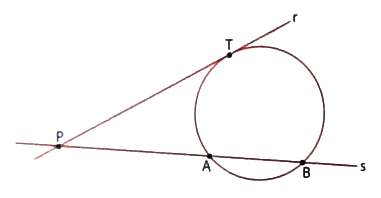
\includegraphics[width=1\linewidth]{imagens_8FMA110/imagem1}
    	\noindent\textsubscript{~---------------------------------------------------------------------------}
    	\begin{enumerate}
    		\item Demonstre a relação anterior. \\\\\\\\\\\\\\\\\\\\\\\\\\\\\\\\\\\\\\
    		\item No desenho a seguir, $\overline{PA}$ é tangente à circunferência no ponto A. \\
    		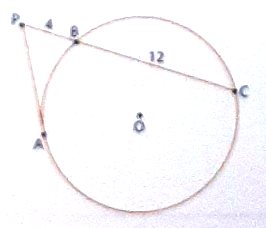
\includegraphics[width=1\linewidth]{imagens_8FMA110/imagem2}
    		\begin{enumerate}[a)]
    			\item Calcule $PA$ \\\\\\\\\\\\\\\\\\\\
    			\item Determine o diâmetro da circunferência, sabendo que $m(A\hat{P}O) = 30^\circ$.\\\\\\\\\\\\\\
    		\end{enumerate}
    		\item Calcule os valores de $x$ nas figuras a seguir, considerando $\overline{PT}$ tangente às circunferências no ponto $T$: \\
    		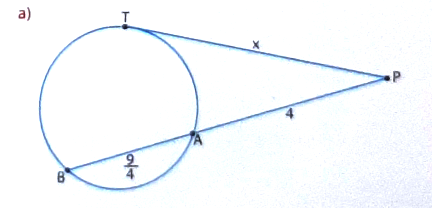
\includegraphics[width=1\linewidth]{imagens_8FMA110/imagem3} \\\\\\\\\\\\\\\\\\\\\\\\\\\\
    		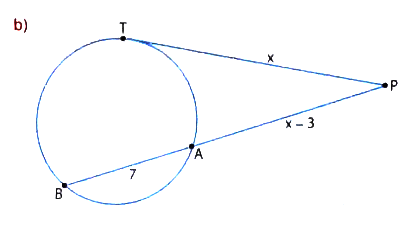
\includegraphics[width=1\linewidth]{imagens_8FMA110/imagem4}
    		\columnbreak
    		\item Sabemos que a média geométrica dos números positivos é $a$ e $b$ é o número positivo $x$ tal que $x^2 = ab$. Usando régua e compasso, ache um segmento cuja medida é a média geométrica dos segmentos dados a seguir.
    		\textbf{Observação:} a hipotenusa de um triângulo retângulo inscrito numa circunferência é um diâmetro dessa circunferência. \\
    		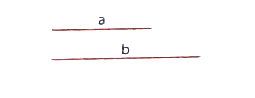
\includegraphics[width=1\linewidth]{imagens_8FMA110/imagem5}
    		\newpage
    		\item Uma fazenda circular possui três portões, localizados nos pontos $A, B$ e $C$. A rua $X$, tangente à fazenda no portão $A$, cruza a rua $Y$ no ponto $P$, onde se localiza um posto de gasolina, como mostra a figura a seguir. \\
    		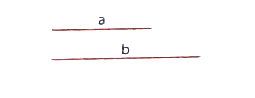
\includegraphics[width=1\linewidth]{imagens_8FMA110/imagem5}
    		Para ir ao posto de gasolina, o dono da fazenda precisa percorrer 4 km caso escolha sair pelo portão $C$. Sabendo que a distância entre os portões $B$ e $C$ é de 5 km, qual a distância que o dono percorreria até o posto de gasolina caso optasse sair pelo portão $A$? \\\\\\\\\\\\\\\\\\\\\\\\\\\\\\\\\\\\\\\\\\\\
    		\textbf{Desafio olímpico} \\\\
    		Os comprimentos $XP$ e $AO$, indicados na figura, são 6 cm e 8 cm, respectivamente. \\
    		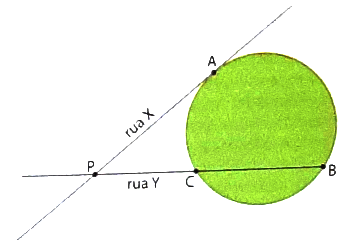
\includegraphics[width=1\linewidth]{imagens_8FMA110/imagem6} \\
    		Qual a medida de $\overline{XB}$?
    		\begin{enumerate}[a)]
    			\item 15 cm
    			\item 13 cm
    			\item 10 cm
    			\item 6 cm
    			\item 2 cm
    		\end{enumerate}
    	\end{enumerate}
    $~$ \\ $~$ \\ $~$ \\ $~$ \\ $~$ \\ $~$ \\ $~$ \\ $~$ \\ $~$ \\ $~$ \\ $~$ \\ $~$ \\ $~$ \\ $~$ \\ $~$ \\ $~$ \\ $~$ \\ $~$ \\ $~$ \\ $~$ 
    \end{multicols}
\end{document}